\chapter{Pruebas}

En este capítulo, se detallará el proceso de verificación del correcto funcionamiento de la plataforma a través de pruebas unitarias y de integración. 

Describiremos cómo se diseñaron y ejecutaron estas pruebas para garantizar que cada módulo del sistema funcione de manera correcta y que la interacción entre los distintos componentes sea fluida y eficiente. 

Asimismo se abordarán las herramientas y marcos de prueba utilizados, así como los métodos para identificar y corregir posibles errores o inconsistencias. 

Igualmente se discutirán las pruebas de rendimiento, seguridad y usabilidad, evaluando cómo la plataforma responde bajo diferentes condiciones y garantizando una experiencia de usuario óptima.  

\newpage

\section{Pruebas en la \textit{base de datos}}

Para verificar inicialmente el correcto funcionamiento de la base de datos, se utilizó \texttt{mongosh}, la consola interactiva de MongoDB. Se realizaron pruebas básicas para comprobar que el script de instalación creaba correctamente la base de datos y la colección correspondiente.

Además, se llevaron a cabo operaciones de inserción, eliminación y actualización de documentos, evaluando el comportamiento esperado del sistema. A medida que avanzaba el desarrollo del \textit{backend} y el \textit{frontend}, se continuó comprobando que las interacciones con la base de datos se realizaban correctamente, esta vez a través de los métodos implementados en cada uno de estos módulos.

\newpage

\section{Pruebas en el \textit{backend}}

Para realizar pruebas en el \textit{backend}, se utilizó \textbf{Swagger}, una herramienta que permite visualizar y probar de forma interactiva las rutas de una API. Swagger facilita la documentación automática de las APIs RESTful, y en este caso fue generada automáticamente por \texttt{FastAPI}, el framework utilizado para el desarrollo del servidor.

Gracias a Swagger, accesible en la dirección \href{http://localhost:8000/docs\#/}{http://localhost:8000/docs\#/}, se pudieron ejecutar pruebas para cada uno de los endpoints definidos, especificando los campos requeridos, el cuerpo en formato \texttt{JSON} en caso de ser necesario, y visualizando tanto las respuestas del servidor como los posibles errores. Además el propio uvicorn cuando se ejecuta muestra que métodos ejecuta y los errores que ocurren.

Durante el desarrollo, se fue comprobando el correcto funcionamiento de cada uno de los métodos a través de esta interfaz. Esto permitió detectar y corregir errores de manera ágil, gracias a la retroalimentación inmediata proporcionada por la API. Asimismo, se realizaron pruebas introduciendo datos erróneos de forma intencionada con el objetivo de evaluar la robustez del sistema ante entradas inválidas o inconsistentes.

También se simularon escenarios de fallo como la indisponibilidad de los modelos de lenguaje —por ejemplo, debido a un exceso de tokens o a errores en el nombre del modelo— para verificar cómo respondía el sistema en situaciones excepcionales.

Posteriormente, durante el desarrollo del \textit{frontend}, las pruebas comenzaron a realizarse principalmente desde la propia interfaz de usuario. No obstante, en ciertas ocasiones se continuó utilizando Swagger para llevar a cabo pruebas rápidas y directas sobre los endpoints.

\begin{figure}[H]
	\centering
	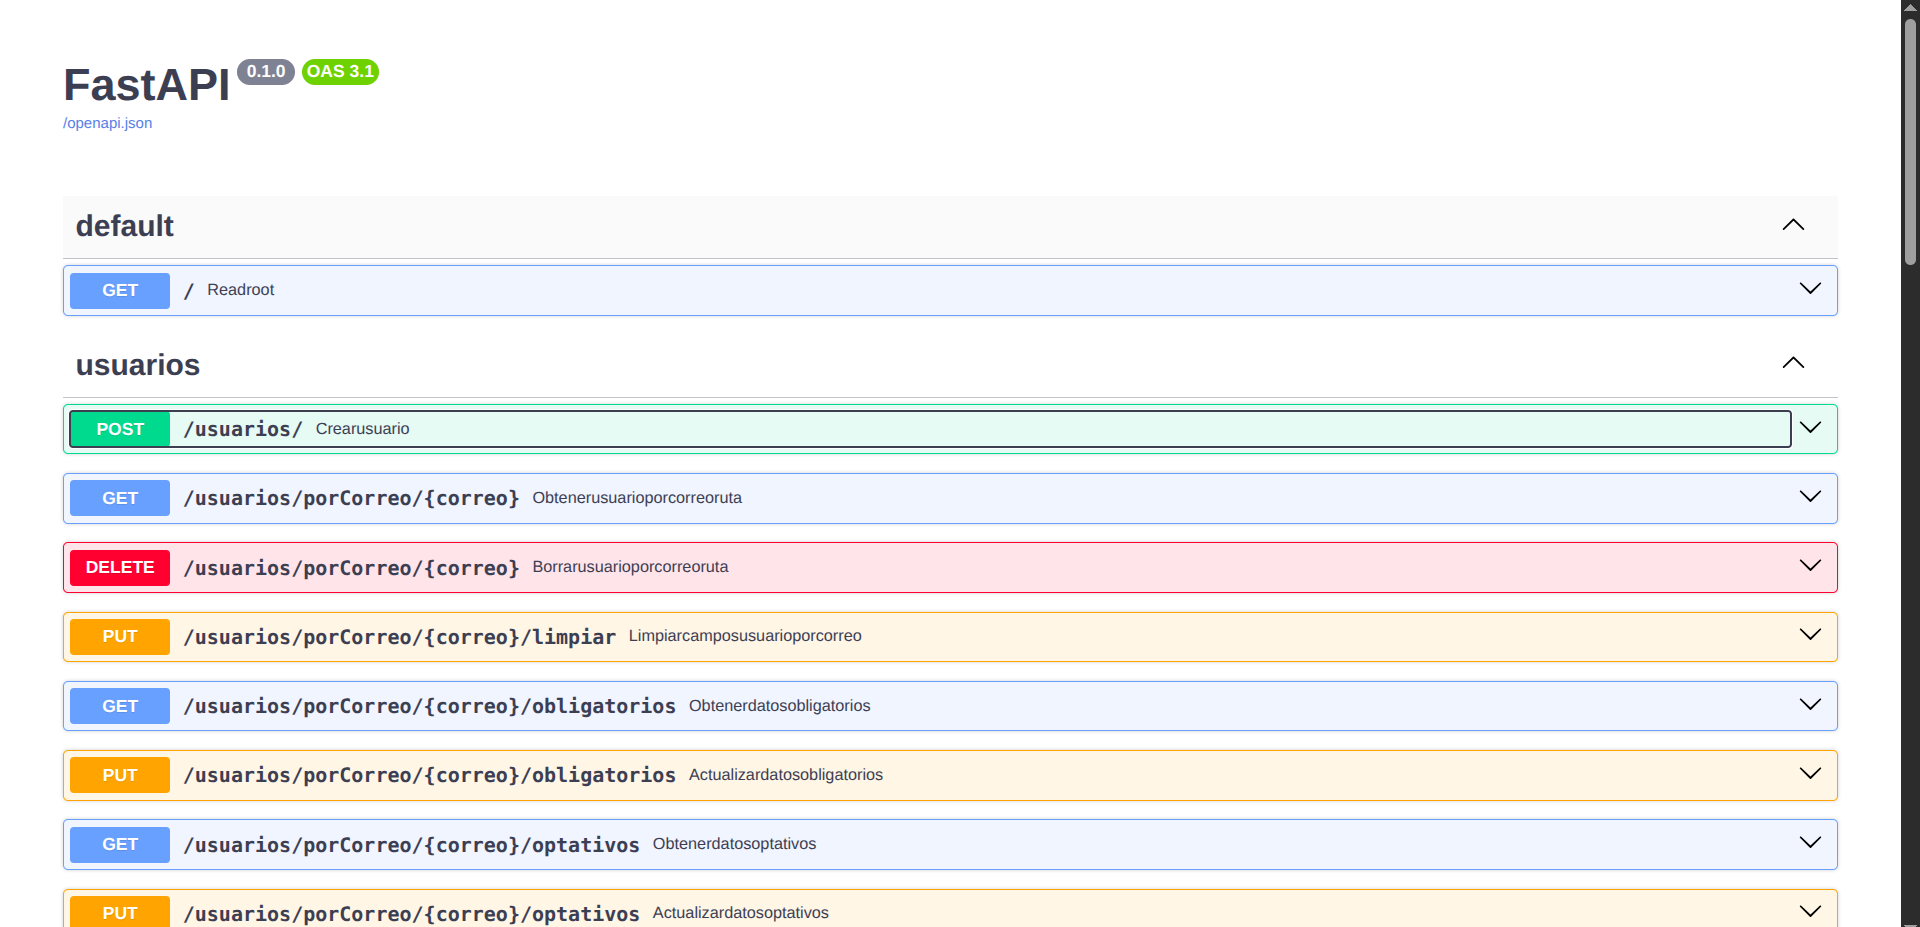
\includegraphics[width=1\linewidth]{imagenes/swagger1.png}
	\caption[\textbf{Vista general de Swagger}.]{\textbf{Vista general de Swagger}. Vista general de la API generada por Swagger a partir del código de FastAPI.}
	\label{swagger-1}
\end{figure}

\begin{figure}[H]
	\centering
	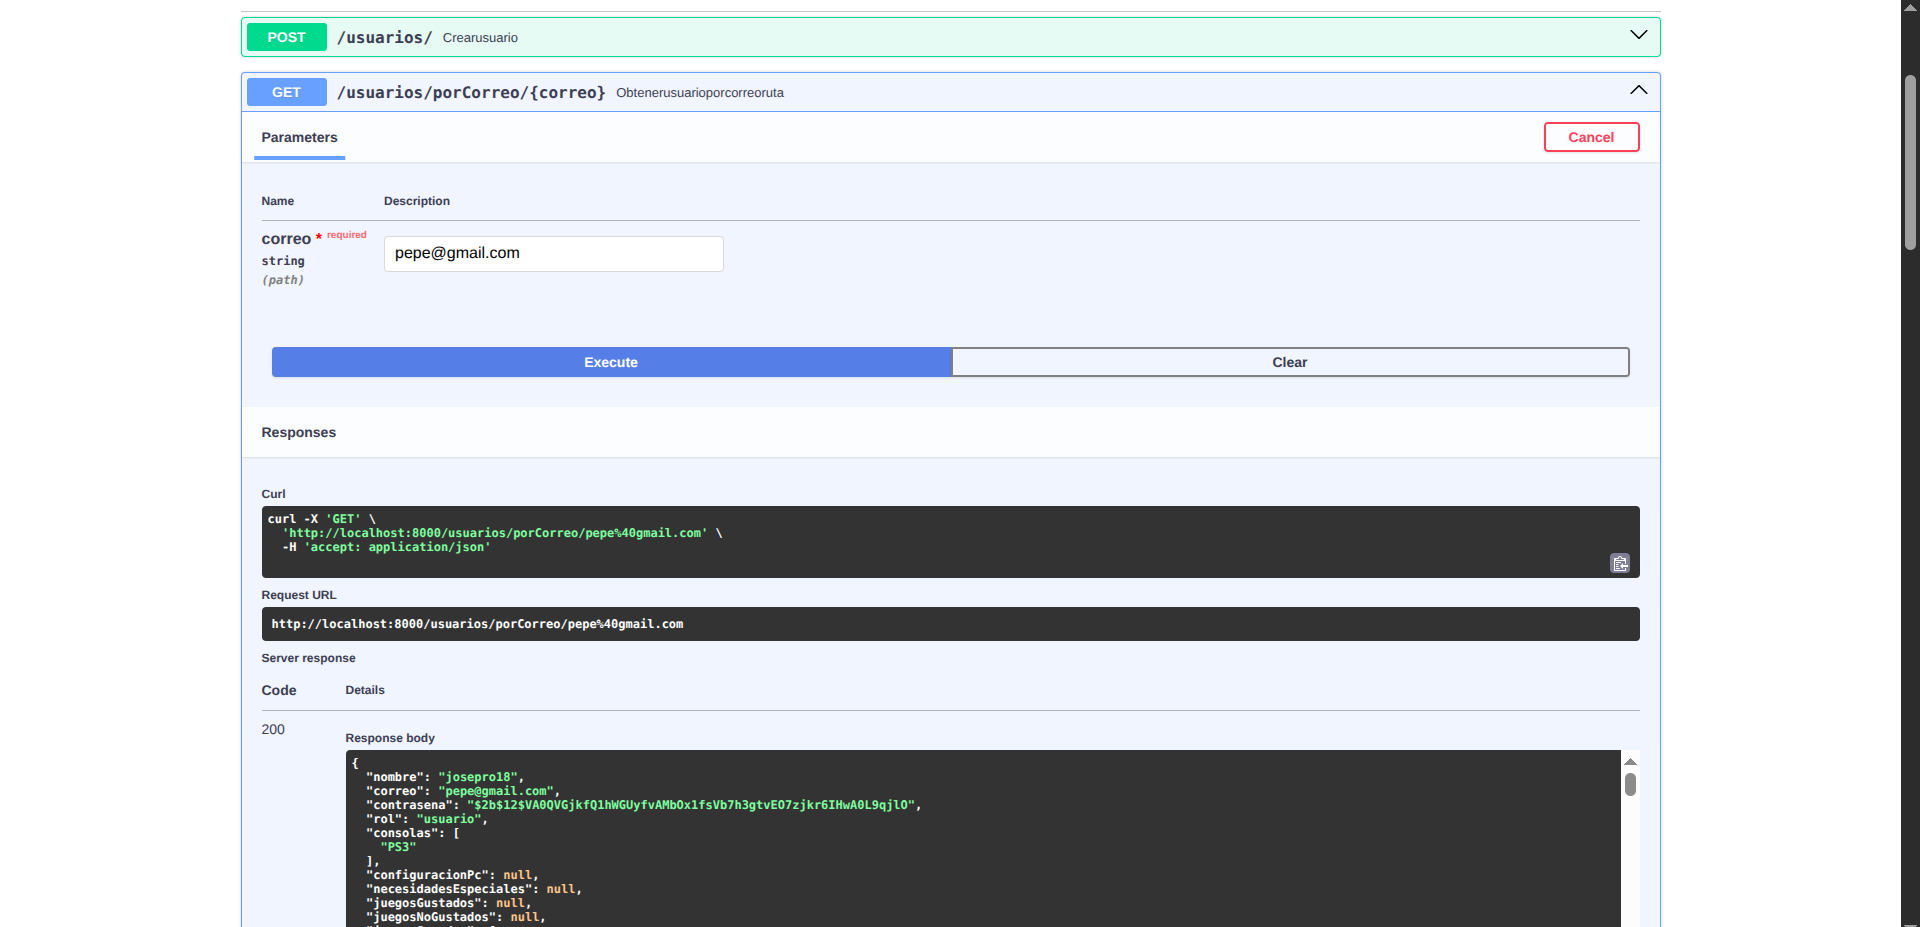
\includegraphics[width=1\linewidth]{imagenes/swagger2.png}
	\caption[\textbf{Vista del uso de un método en Swagger}.]{\textbf{Vista del uso de un método en Swagger}. Se muestra el método \texttt{GET} para obtener un usuario, al que se le pasa el correo electrónico como parámetro, devolviendo un \texttt{JSON} con los datos del usuario.}
	\label{swagger-2}
\end{figure}

\subsection{Pruebas unitarias y de integración en el \textit{backend}}

Además de las pruebas realizadas con Swagger, se han desarrollado pruebas unitarias e integradas para el módulo de \textit{backend} utilizando la librería \texttt{unittest} junto con \texttt{mongomock}, una herramienta que simula el comportamiento de una base de datos MongoDB en memoria. Esto permitió realizar pruebas sin necesidad de conectarse a una base de datos real.

Estas pruebas se organizaron en dos ficheros separados dentro de una carpeta \texttt{test}: un archivo para gestionar usuario y otro para la autentificación. El primero contiene pruebas sobre la lógica de gestión de usuarios, mientras que el segundo verifica las rutas de autenticación expuestas por la API de FastAPI.

Las funciones principales del sistema se comprobaron de forma individual, incluyendo la creación, actualización, eliminación y verificación de usuarios. Para ello, se prepararon entornos simulados en cada prueba, creando una base de datos ficticia e inyectando los datos necesarios para comprobar el comportamiento del sistema. También se emplearon técnicas de \textit{mocking} para simular el comportamiento de las funciones de encriptación de contraseñas (\texttt{bcrypt}) y de generación de tokens JWT, permitiendo centrarse en la lógica del sistema sin depender de funcionalidades externas.

En el caso de las rutas de autenticación, se utilizó \texttt{TestClient}, un cliente de pruebas proporcionado por FastAPI, para simular peticiones HTTP y verificar las respuestas del servidor. Se probaron casos como el inicio de sesión con credenciales correctas, contraseñas incorrectas y usuarios inexistentes, evaluando la respuesta del sistema ante distintos escenarios.

Estas pruebas automáticas permiten garantizar que los métodos clave del \textit{backend} funcionan correctamente, tanto de forma aislada como cuando interactúan entre sí. Además, al ejecutarse de manera repetida, facilitan la detección temprana de errores ante futuros cambios en el código.

\newpage

\section{Pruebas en el \textit{frontend}}

Para llevar a cabo las pruebas en el \textit{frontend}, se inicializó el servidor de Angular y se accedió a la dirección local \href{http://localhost:4200/}{http://localhost:4200/}. Desde esta interfaz se realizaron pruebas interactivas explorando todos los elementos visibles, accionando botones y navegando por los distintos componentes de la aplicación.

La detección de errores se realizaba principalmente a través de dos vías: por un lado, mediante los mensajes devueltos por la API en caso de errores de validación o fallos internos; por otro, mediante el uso de las herramientas de desarrollo del navegador. Estas herramientas, accesibles pulsando \texttt{F12}, permiten inspeccionar múltiples aspectos del comportamiento del sitio web.

En particular, se hizo uso de la \textbf{consola del navegador}, que permite visualizar errores de ejecución de Angular, advertencias, trazas de red, y mensajes de depuración. También se utilizó la pestaña de herramientas de \textit{responsive design}, que simula el comportamiento de la interfaz en diferentes tamaños de pantalla, permitiendo verificar que la aplicación mantiene su usabilidad y legibilidad tanto en dispositivos móviles como en pantallas de escritorio.

\begin{figure}[H]
	\centering
	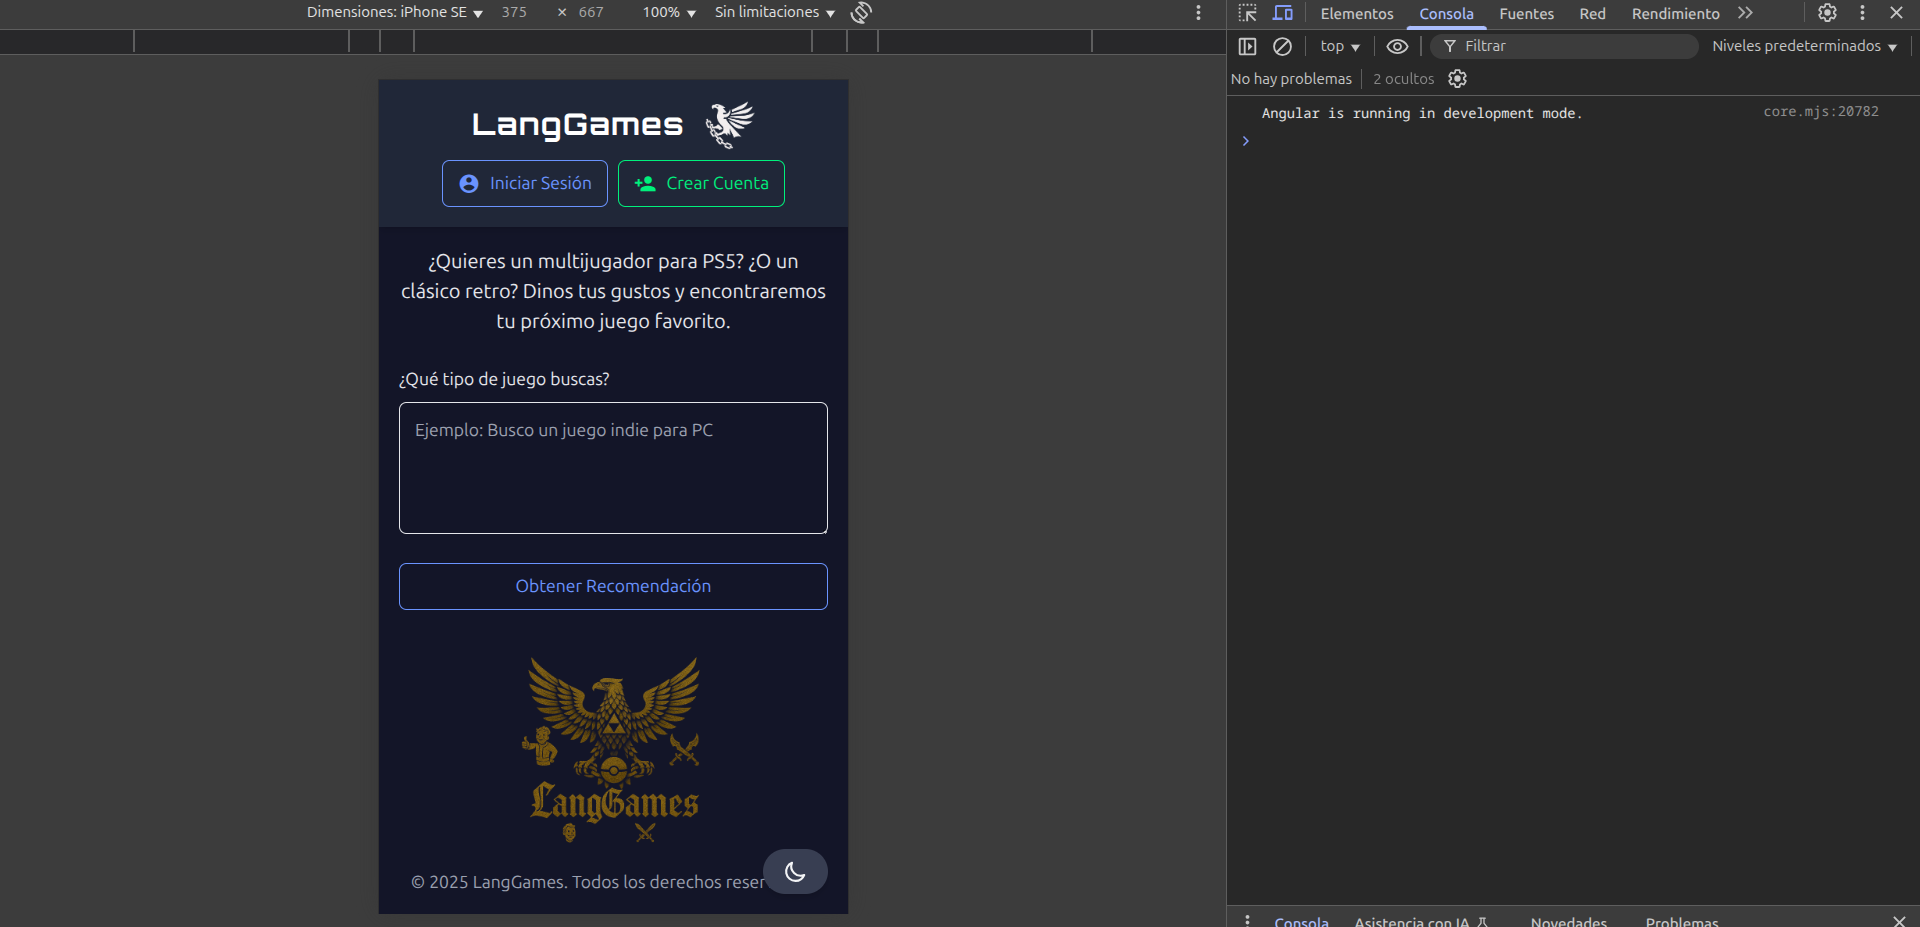
\includegraphics[width=1\linewidth]{imagenes/consolaNavegador.png}
	\caption[\textbf{Vista de las herramientas de desarrollo del navegador}.]{\textbf{Vista de las herramientas de desarrollo del navegador}. Estas herramientas permiten detectar errores de Angular y comprobar que el diseño es adaptable a distintos dispositivos.}
	\label{consola-navegador}
\end{figure}

\newpage

\section{Pruebas extras}

Para asegurar una mejor robustez de la plataforma, se ha realizado una instalación de la aplicación en una máquina virtual de Ubuntu nueva, lo que permitió corregir errores que no se vieron durante el desarrollo por instalar las cosas una por una. 

Por ejemplo, la primera vez que se lanza angular se pide al usuario que especifique ciertas preferencias, pero al lanzarse en segundo plano el usuario no podía elegir. Para paliar este problema se realiza un primer lanzamiento de angular en primer plano después de la aplicación.


Además se ha compartido el proyecto con un compañero de informática de la universitat oberta de Catalunya para que pruebe la aplicación y de sus conclusiones. 

\newpage

\section{Conclusión}

A lo largo de este capítulo se ha descrito el proceso de pruebas llevado a cabo para verificar el correcto funcionamiento de cada uno de los módulos de la plataforma.

En primer lugar, se realizaron pruebas directas sobre la base de datos mediante \texttt{mongosh}, asegurando que las operaciones básicas de inserción, actualización y eliminación funcionaban correctamente. Posteriormente, se probó el \textit{backend} utilizando Swagger, lo que permitió evaluar de forma precisa cada uno de los endpoints expuestos por la API, simulando tanto casos correctos como situaciones de error o fallo del sistema.

Finalmente, el \textit{frontend} fue validado mediante interacción directa con la aplicación y mediante el uso de las herramientas de desarrollo del navegador, lo cual permitió no solo identificar errores de ejecución, sino también comprobar la adaptabilidad del diseño a distintos dispositivos.

Este enfoque integral de pruebas, que abarca desde el nivel más bajo (base de datos) hasta el más alto (interfaz de usuario), ha permitido garantizar una plataforma funcional, robusta y preparada para ofrecer una experiencia de usuario óptima. Además, se ha verificado que los distintos componentes interactúan de forma fluida, cumpliendo con los requisitos del sistema.

